\subsection{The Plan and The Sphere}

In the plane, if one scales a polygon, the area of the polygon changes
but the angles of the polygon do not change.
On the unit sphere, we can relate the area of a simple polygon 
to the angles. This is because the sphere is curved.
A triangle on the sphere is shown in \figref{sphere-triangle}.


 \begin{figure}[htb]
         \centering
        \begin{subfigure}[b]{0.35\textwidth}
         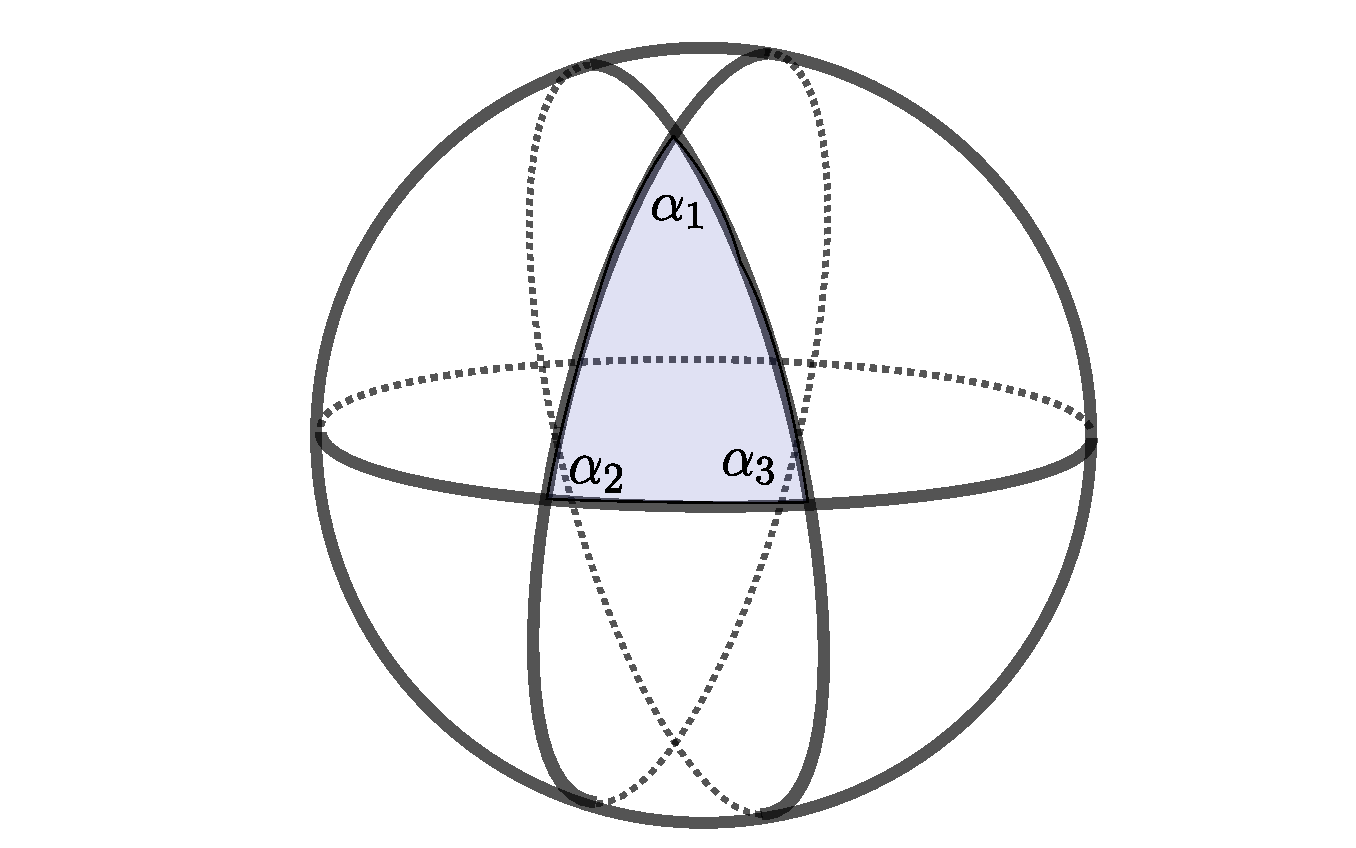
\includegraphics[width=\textwidth]{background/sphere-triangle}
         \caption{Spherical triangle.}
 	 \label{fig:sphere-triangle}
       \end{subfigure}
         \hspace{1cm}
         \begin{subfigure}[b]{0.35\textwidth}
         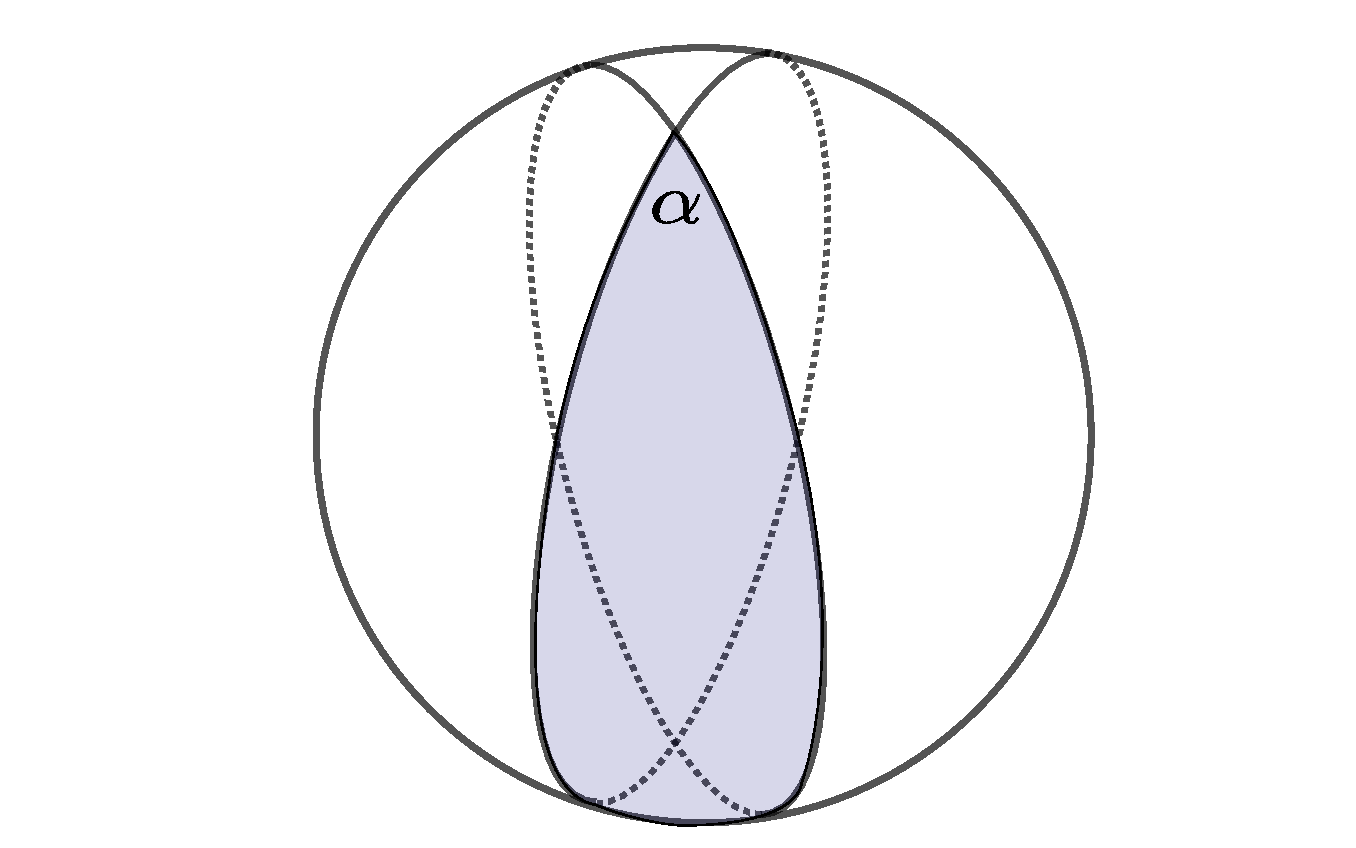
\includegraphics[width=\textwidth]{background/lune}
         \caption{A lune.}
          \label{fig:lune}
         \end{subfigure}
		\caption{(a) A triangle on the sphere.
 		(b) A lune with angle $\alpha$.
 		\label{fig:sphere-lune}}
 \end{figure}
A spherical \EMPH{lune} is the region on a sphere bounded by two half great circles
with angle $\alpha$. The area of a lune is denoted $A(\alpha)$,
 see \figref{lune}.
On the unit sphere, the area of a lune is proportional to $\alpha$. 
If $\alpha=0$ the area is zero and if $\alpha=\pi$ the area is $4\pi$.
We can add the area of two lunes in terms of their angles, 
$A(\alpha_1+\alpha_2)=A(\alpha_1)+A(\alpha_2)$ so $A$ is linear
and  $A(\alpha)=4\alpha.$




The following relates the area of a triangle on the sphere to the angles.

\begin{lemma}[Area of Spherical Triangle]\label{lem:spherical-triangle}
On the unit sphere, the area of a triangle with interior angles $\alpha_1, \alpha_2, \alpha_3$
is $A=\alpha_1+\alpha_2+\alpha_3-\pi$.
\end{lemma}

\begin{proof}
	Any two edges of the the triangle form a lune. The collection of 
	all three lunes covers the entire sphere with triangle and the antipodal triangle covered three times.
 	The surface area of the unit sphere is $4\pi$.
	Thus, $4\pi=4\alpha_1+4\alpha_2+4\alpha_3-4A$
	and $A=\alpha_1+\alpha_2+\alpha_3-\pi$.
\end{proof}

As in the plane, any polygon on the sphere with $n$ vertices can be decomposed
into $n-2$ triangles \cite{orourke_computational_1994}. This gives a formula for the area of a simple polygon
on the sphere with interior angles $\alpha_1,\alpha_2,\ldots, \alpha_n$.

\begin{equation} \label{eqn:sphere-area}
	A=(2-n)\pi +\sum_{i=1}^n \alpha_i.
\end{equation}





What  do we require of a definition of curvature?
A straight line should have zero curvature and
 large circles should have less curvature than smaller circles.
We also need to differentiate between
curving to the left and curving to the right.

For any point on a smooth one dimensional curve in the plane,
we can approximate the curve with a circle.
The best approximating circle is the  \EMPH{osculating circle}.
A natural definition of the \EMPH{curvature} is the inverse of the radius of the osculating
 circle $k=\frac{1}{r}$.
See \figref{osculating-circle} for an example.
The osculating circle meets the requirements for a definition of curvature.
We determine the sign of the curvature by which side of the curve the osculating circle is on.




The above definition provides great intuition for the curvature of curves
and surfaces.
Computing this value depends on how a curve or surface is represented. 

\begin{figure}[htb]
	\centering
	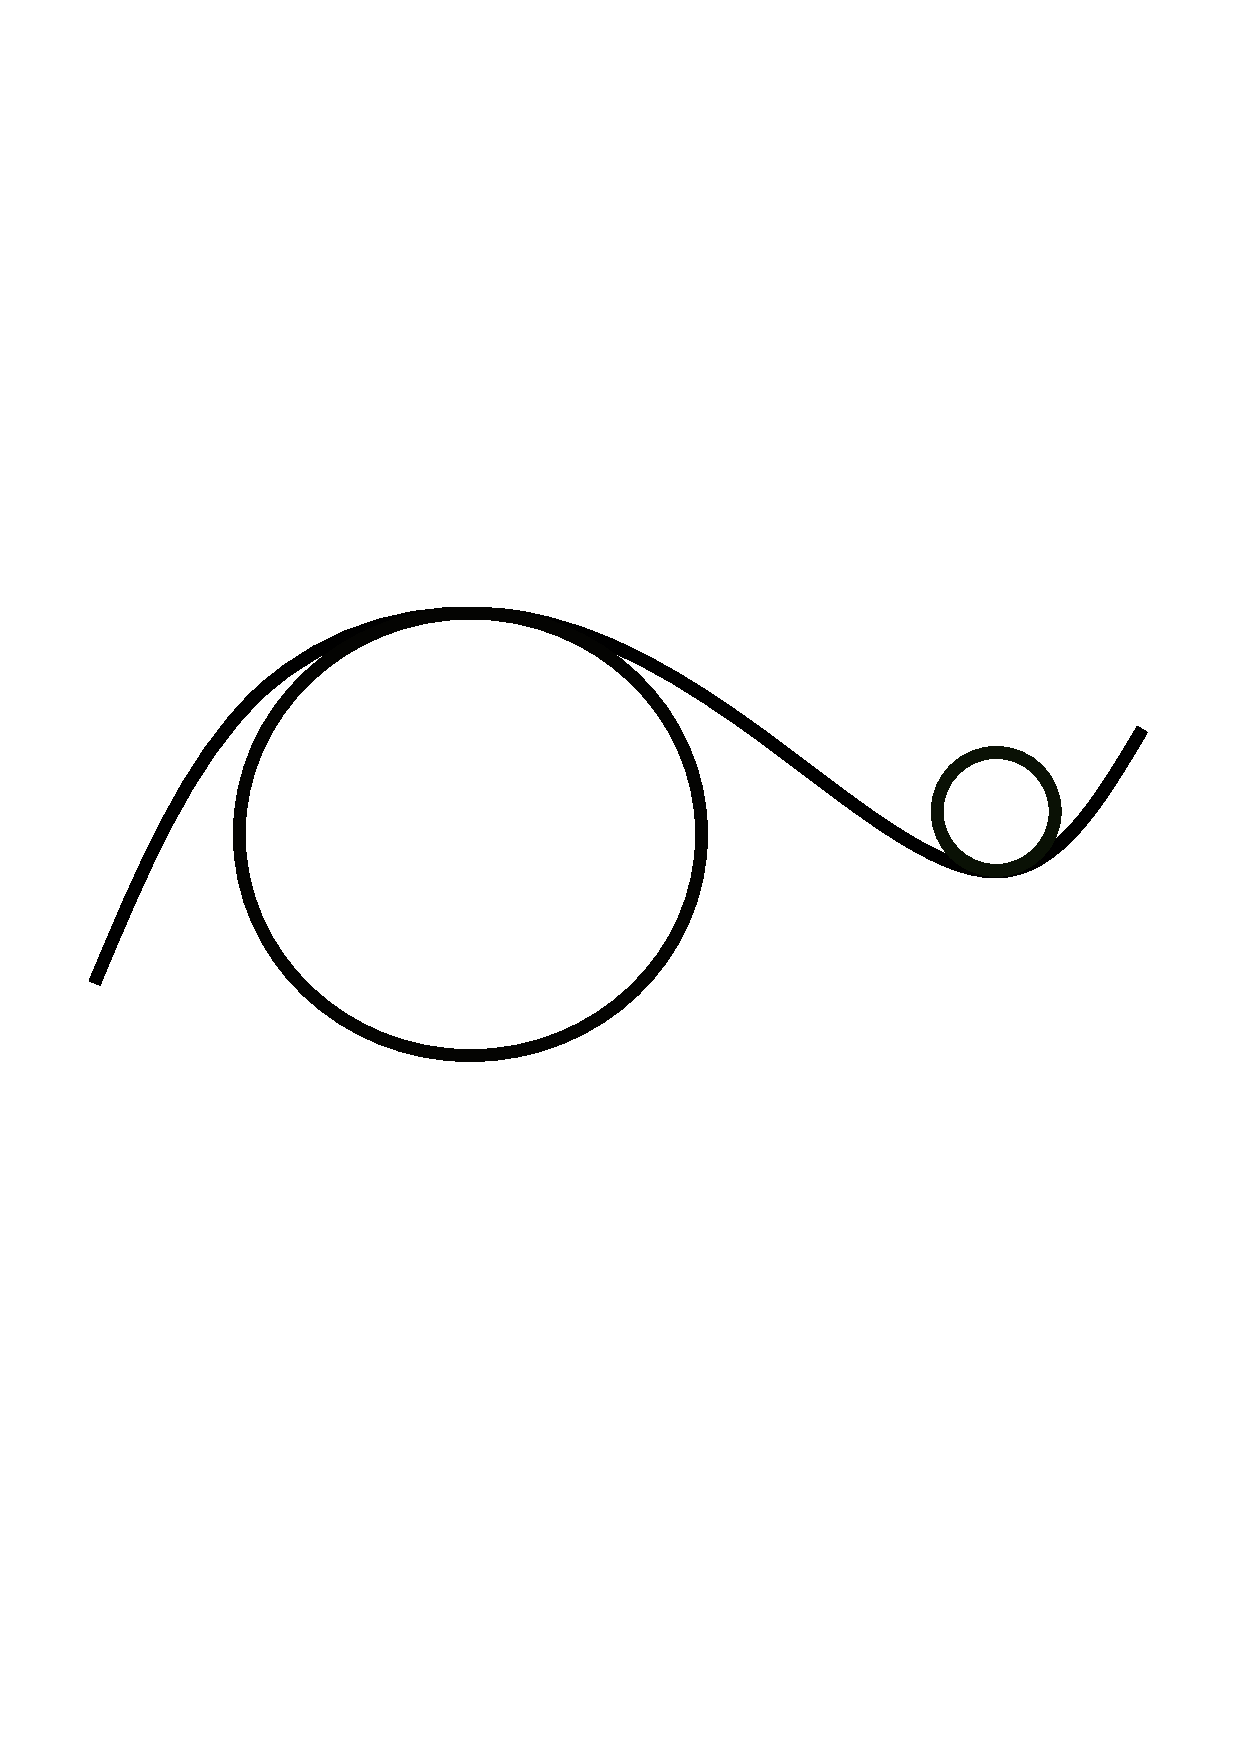
\includegraphics[width=.3\textwidth]{curvature/osculating}
	\caption{A curve with two osculating circles. The curvature at these points
	have opposite sign.}
	\label{fig:osculating-circle}
\end{figure}

A curve in $\RR^3$ is often presented as a function
$\gamma(t)=(x(t),y(t),z(t))$. We say that a curve is \EMPH{smooth} on an open interval $I$
if $\gamma'$ it is continuous and $\gamma'(t)\neq (0,0,0)$ on $I$. 
If $\gamma$ is smooth it has a well-defined unit tangent vector $T(t)=\frac{\gamma'(t)}{|\gamma'(t)|}.$
A second way to define the  \EMPH{curvature} at a point is as the signed magnitude of the rate of change of the 
unit tangent vector

\begin{equation} \label{eqn:kappa}
\kappa= \pm | T'(t)|.
\end{equation}
where $t$ is arc length.

For example, take a circle of radius $r$, parameterized by 
$$C(t)=\left(r\cos(t),r\sin(t),0\right).$$
We have 
$$\frac{dC}{dt}=C'(t)=\left(-r\sin(t),r\cos(t),0\right)$$ and $|C'(t)|=r.$
Then $T(t)=\left(-\sin(t),\cos(t),0\right)$ and
$T'(t)=\left(-\cos(t),-\sin(t),0\right)$.
So, $\kappa(t)=\frac{1}{r}$ and, in this case, our definition of curvature agrees with the
osculating circle intuition given above. 
\eqnref{kappa} can be rewritten in the following more computational friendly form 
\begin{equation} \label{eqn:kappa1}
\kappa(t)=\frac{|\gamma'(t)\times \gamma''(t)|}{|\gamma'(t)|^3}.
\end{equation}

Since we traverse $\gamma$
at unit speed, $\gamma'(t)^2=1,$ and by the chain rule, $\gamma'\cdot \gamma''=0,$
so  the second derivative is orthogonal to $\gamma'$. Thus, the
vector $\gamma''=N$ is normal to the $\gamma$. 
By taking the cross product of $N$ and $T$ we obtain a vector $B$ called
the binormal vector.
The vectors $T,N$ and $B$ form the \EMPH{Fernet frame} of $\gamma$ a $p.$

 This osculating-circle idea can be extend
to  surfaces in $\R^3$, by considering the \EMPH{osculating sphere},
But notice that at saddle points on a surface it is not clear which sphere
best approximates the surface. See \figref{osculating-sphere} for two
equally reasonable ways to approximate a saddle with a sphere.

\begin{figure}[htb]
    \captionsetup[subfigure]{justification=centering}
    \centering
    \begin{subfigure}[b]{0.25\textwidth}
        \includegraphics[width=\textwidth]{curvature/sphere-above-saddle}
       \subcaption{}\label{fig:sphere-above-saddle}
    \end{subfigure}
        \hspace{1cm}
        \begin{subfigure}[b]{0.25\textwidth}
        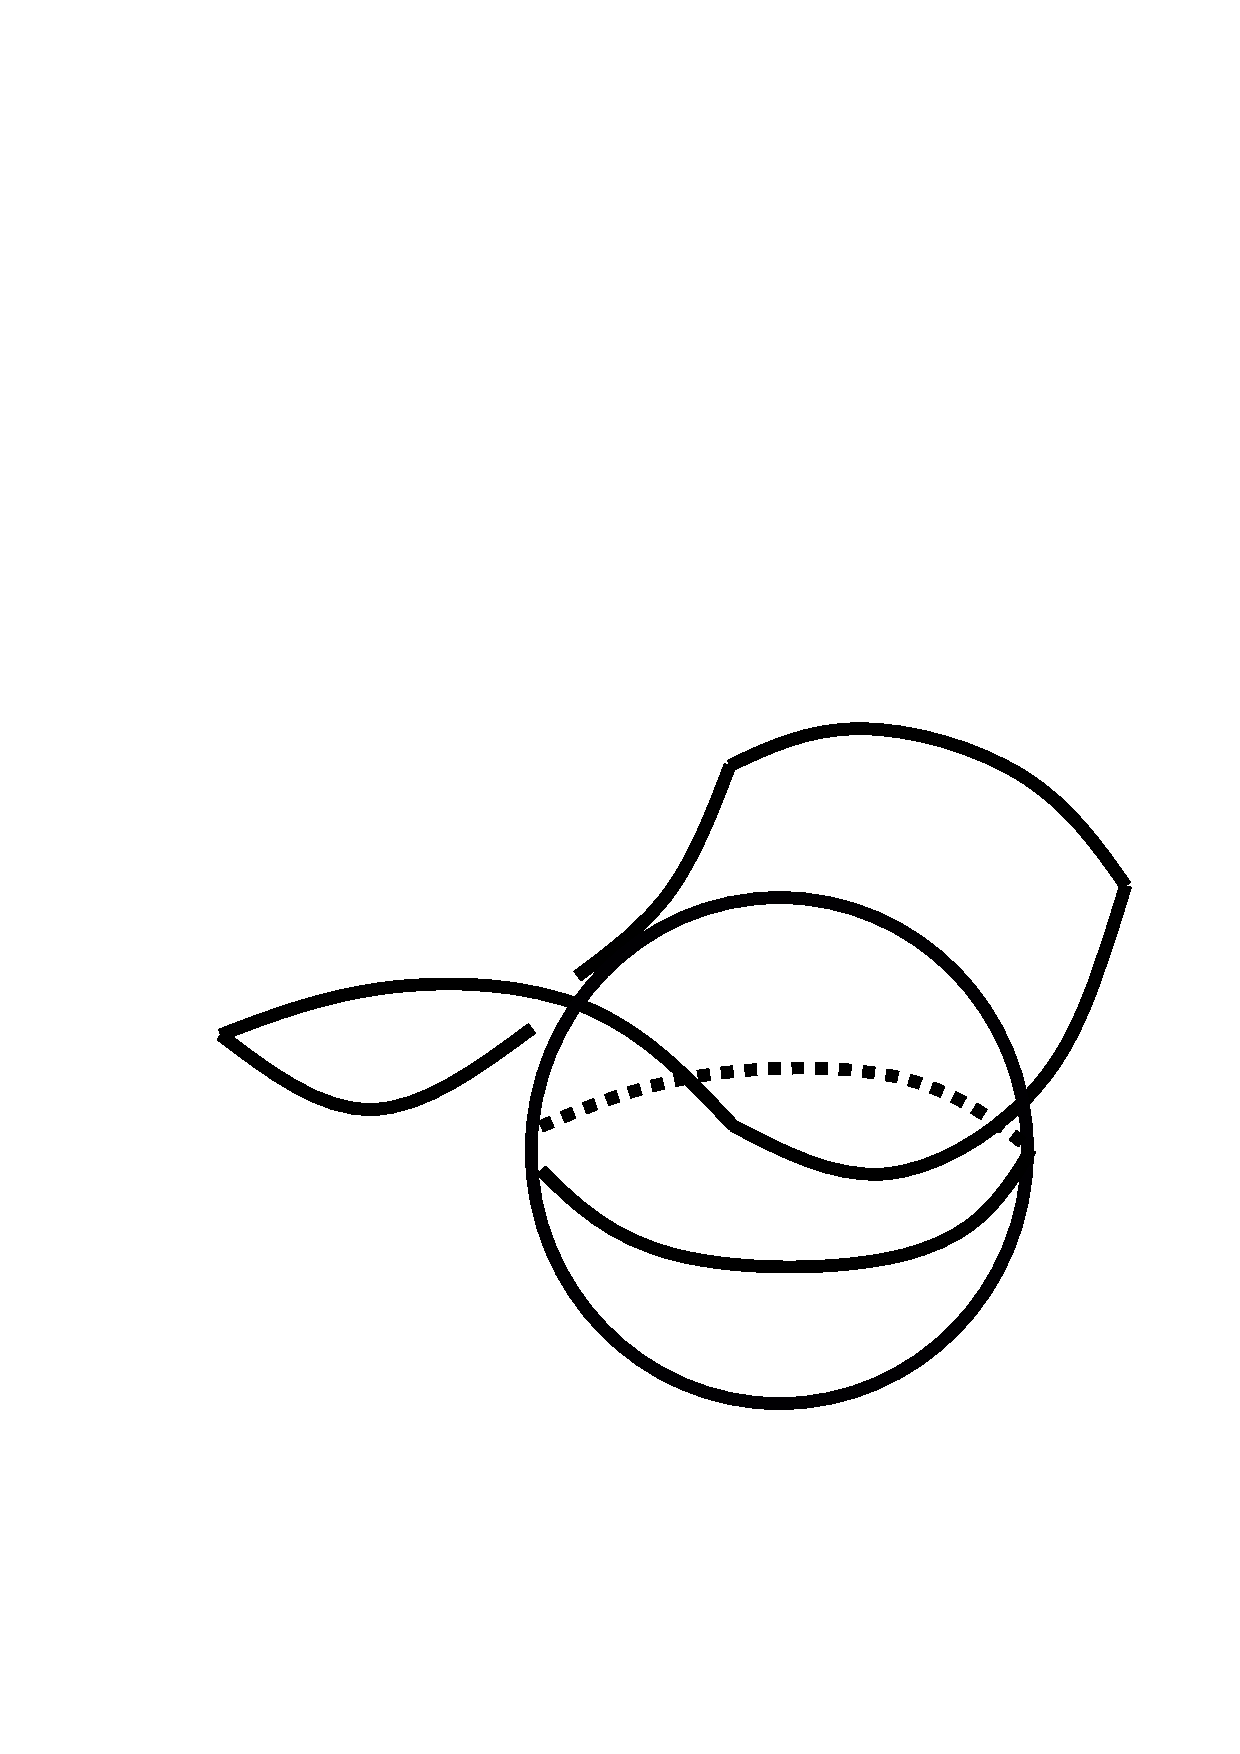
\includegraphics[width=\textwidth]{curvature/sphere-below-saddle}
        \subcaption{}\label{fig:sphere-below-saddle}
        \end{subfigure}
    \caption{(\subref{fig:sphere-above-saddle}) The osculating sphere above the saddle.
        (\subref{fig:sphere-below-saddle}) The osculating sphere above the saddle.
    }
    \label{fig:osculating-sphere}
\end{figure}


Here it is \figref{normal-sections}
\begin{figure}[htb]
    \captionsetup[subfigure]{justification=centering}
    \centering
    \begin{subfigure}[b]{0.25\textwidth}
        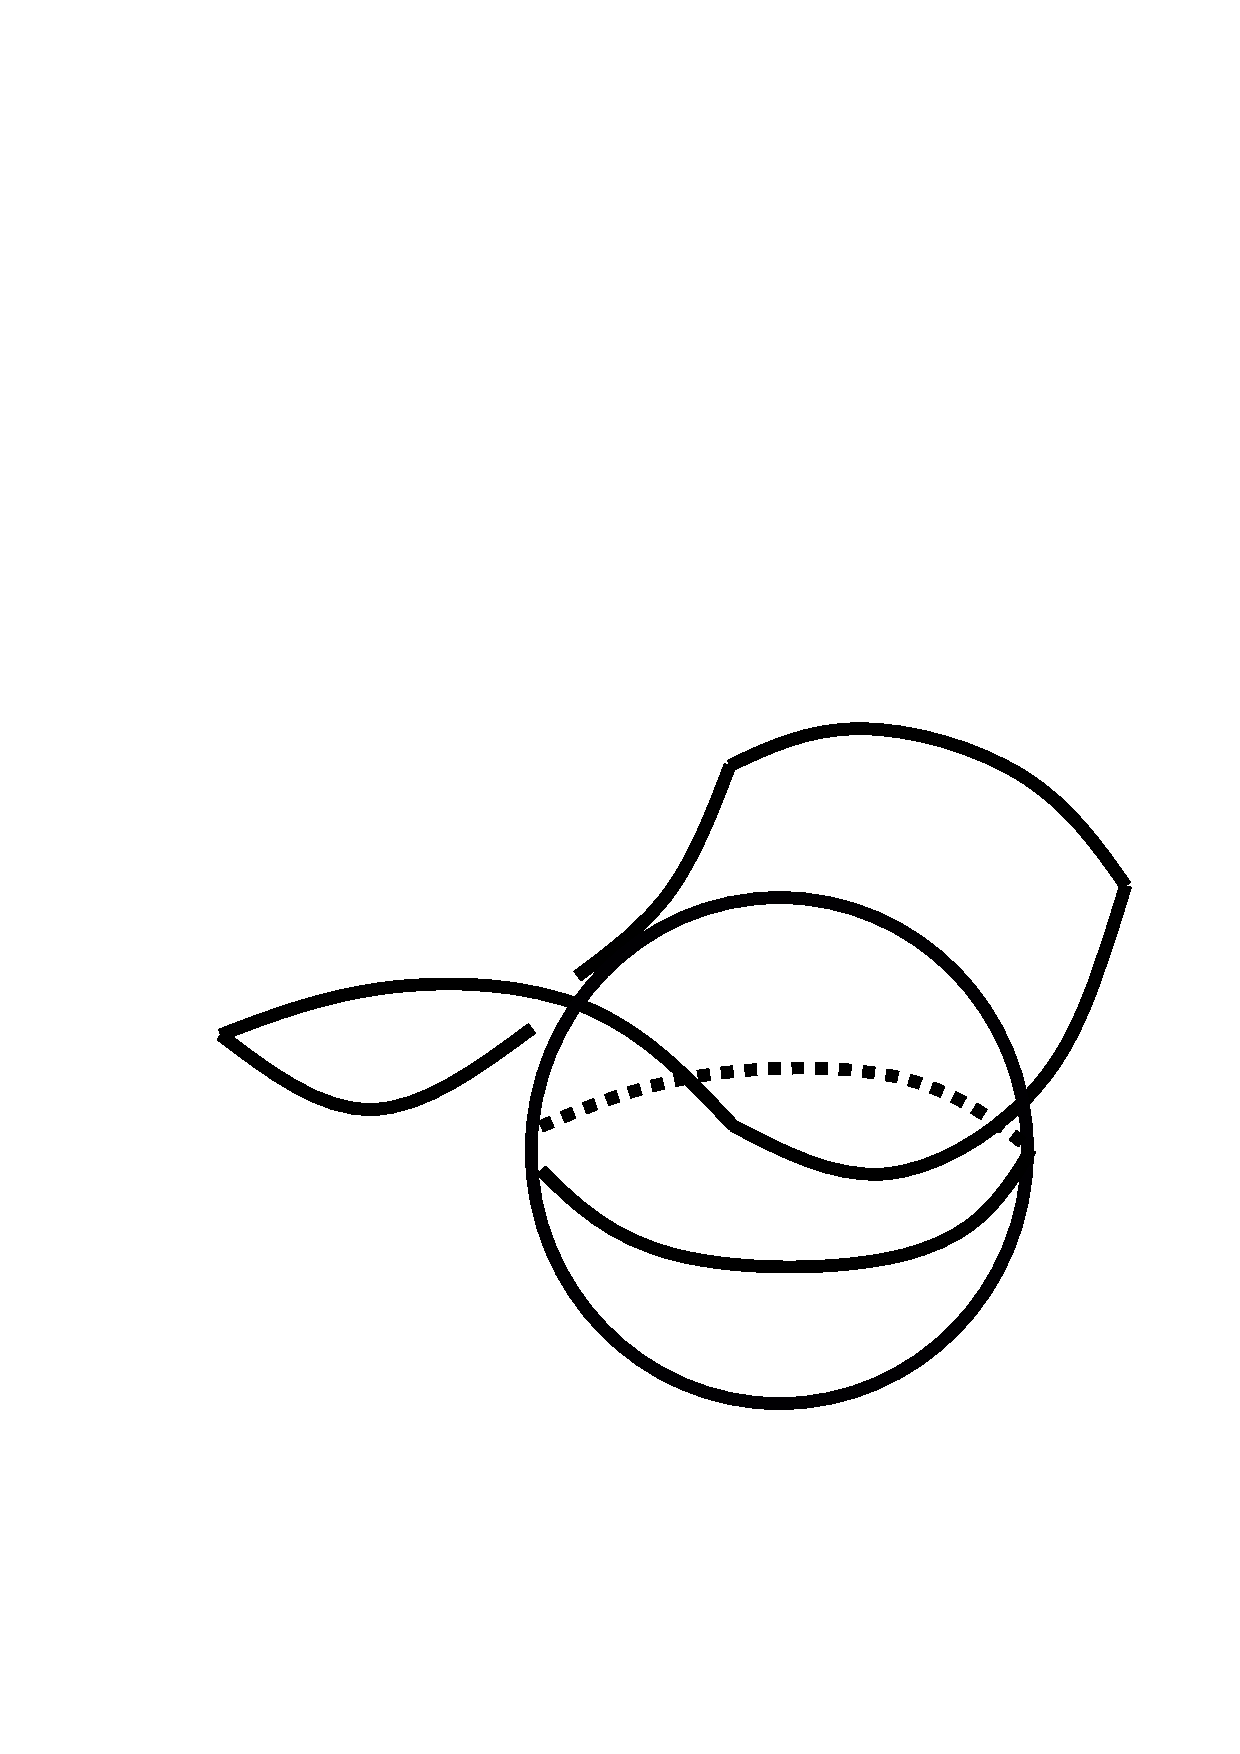
\includegraphics[width=\textwidth]{curvature/normal-section-max}
       \subcaption{}\label{fig:normal-section-max}
    \end{subfigure}
        \hspace{1cm}
        \begin{subfigure}[b]{0.25\textwidth}
        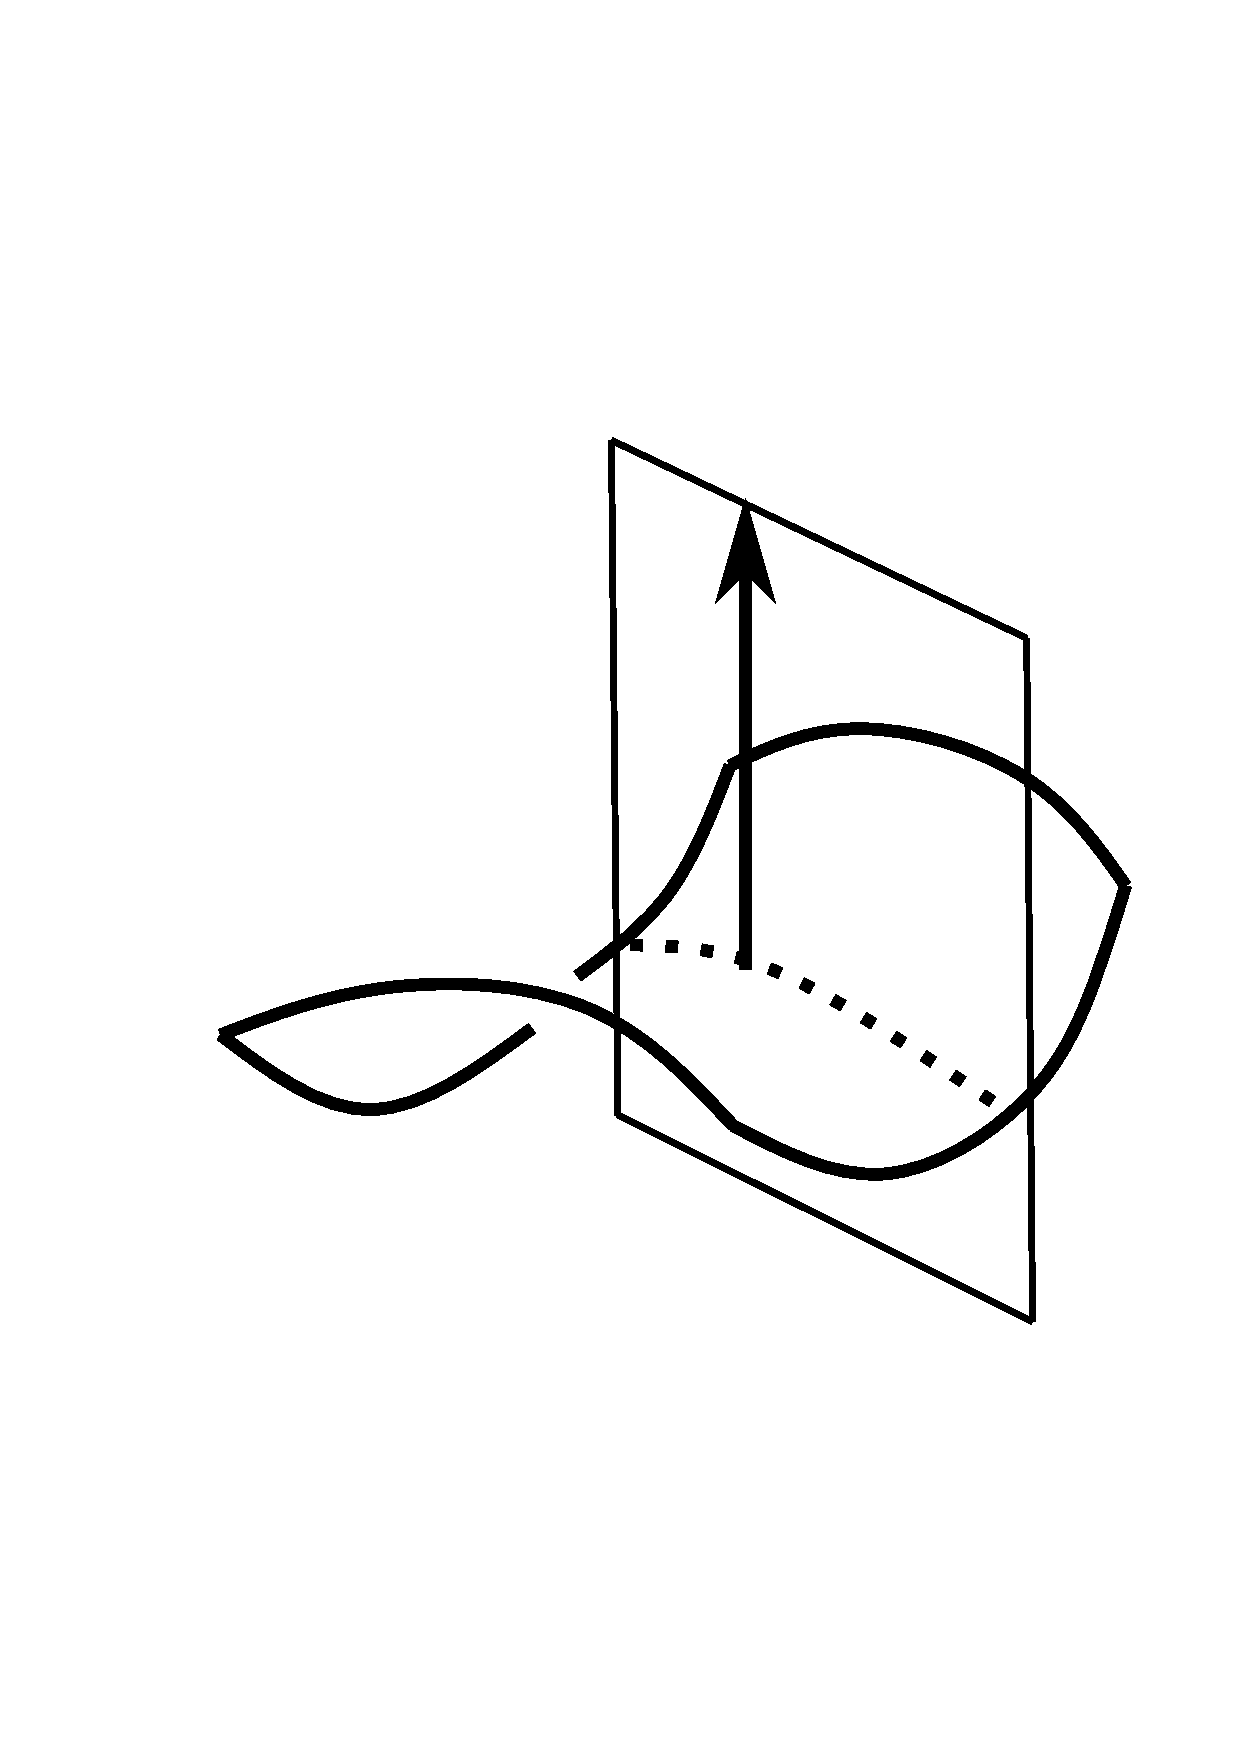
\includegraphics[width=\textwidth]{curvature/normal-section-min}
        \subcaption{}\label{fig:normal-section-min}
        \end{subfigure}
    \caption{(\subref{fig:normal-section-max}) The osculating sphere above the saddle.
        (\subref{fig:normal-section-min}) The osculating sphere above the saddle.
    }
    \label{fig:normal-sections}
\end{figure}

\subsubsection{Surfaces}


One dimensional curves are represented by differentiable 
parameterized functions $\gamma:I\subset \RR\to \RR^3$,
we would now like to parameterize a surface.
Similarly, a \EMPH{parameterized surface} $S$ is a collection of maps such that
 for each point $p\in S$ we have a neighborhood $X\subset S$
 and a map $r:U\subset \RR^2 \to X\subset \RR^3$, $r(u,v)=(x(u,v),y(u,v),z(u,v))$
 where
 \begin{itemize}
 \item  $r$ is a homeomorphism
 \item $r$ has derivatives of all orders
 \item every point in $S$ is contained in the domain of at least one map.

\end{itemize}
The maps in the third item are called \EMPH{charts}.
If the differential $dr_q:\RR^2\to \RR^3$ is one-to-one for all $q\in U$ then
we say $r$ is \EMPH{regular}. In other words, let $(u,v)$ be coordinates of $U\subset \RR^2,$
a surface is regular if $\frac{\partial r}{\partial u}$
and $\frac{\partial r}{\partial v}$ are linearly independent for all $p\in U$.


\begin{example}[The Sphere]\label{ex:sphere-charts}

The unit two sphere $\Sp^2\subset \RR^3$ is the set $\{(x,y,z)\in \RR^3 | x^2+y^2+z^2=1\}.$
We can define six charts to parameterize $\Sp^2$.
For $u,v\in[-1,1]$, we have
$$r_{z}(u,v)=(u,v,\sqrt{1-u^2-v^2}) \hspace{.5cm}  r_{-z}(u,v)=(u,v,-\sqrt{1-u^2-v^2}) \hspace{.5cm}  r_{x}(u,v)=(\sqrt{1-u^2-v^2},u,v) $$
$$r_{-x}(u,v)=(-\sqrt{1-u^2-v^2},u,v) \hspace{.5cm}  r_{y}(u,v)=(u,\sqrt{1-u^2-v^2},v) \hspace{.5cm}   r_{-y}(u,v)=(u,-\sqrt{1-u^2-v^2},v). $$

The chart $r_{z}$ is shown in \figref{sphere-chart}

\begin{figure}[htb]
	\centering
	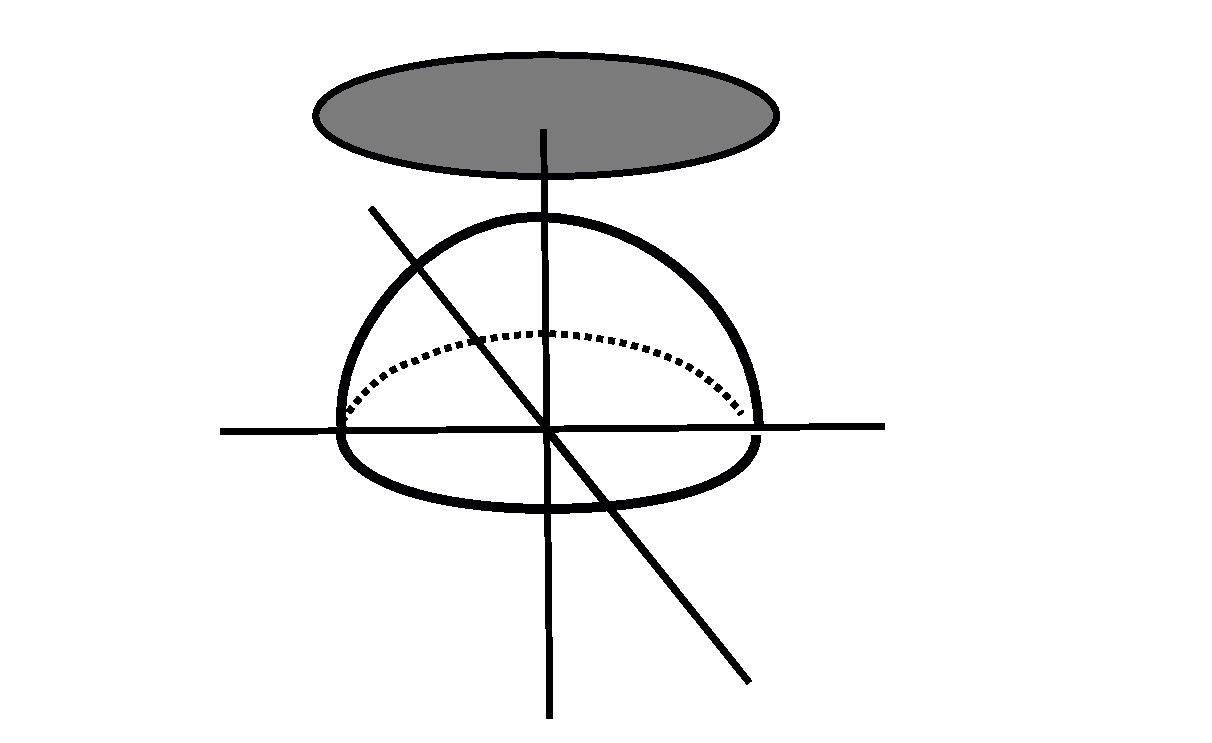
\includegraphics[width=.4\textwidth]{curvature/sphere-chart}
	\caption{A chart of $\Sp^2$.}
	\label{fig:sphere-chart}
\end{figure}

One can verify that these parameterizations fullfil the requirements
for the sphere to be a regular surface.

\end{example}


A \EMPH{tangent vector} to $S$ at $p$ is a map $\xi:(-\epsilon,\epsilon)\to S$ with $\xi(0)=p$.
The set of all tangent vectors is the \EMPH{tangent plane} and it corresponds to the image
of the differential map $d\phi_q(\RR^2)\subset \RR^3$ (prop. 1 \cite{doc76}).
By choosing two linearly independent paths through $p\in S$ we obtain a basis 
for the tangent
plane and define a normal vector $N$ at $p$.
Every plane containing the normal vector will intersect the surface.
The intersection of the surface and each normal plane is a curve in $\RR^3$
gives a one dimensional curve called the \EMPH{normal section}. 
Let $\kappa_1$ denote the maximum curvature of all normal sections 
and let $\kappa_2$ denote the minimum. 
The \EMPH{Gaussian curvature} of a point on a surface is
$K=\kappa_1\kappa_2.$
One can check that the Gaussian curvature of the plane is zero and
that larger circles have less curvature than smaller ones.

Once we choose a chart we define a clockwise orientation to be positive.
 If the clockwise
orientation can be consistently extended to the entire surface, we say
the surface is \EMPH{orientable}.
In one dimension, the curvature is the rate of change of the tangent vector.
For an orientable surface $S$, we consider the rate of change of the normal vector.
This vector is given by the map  $N:S\to \Sp^2$ that sends each
normal in $S$ to the corresponding point on $\Sp^2$ is
the \EMPH{Gauss map}.
The determinant of the derivative of the Gauss map, $dN(p)$ quantifies the rate of change of
the normal vector ($dN$ is often called the \emph{Weingarten map} \cite{Crane:2013}).
Thus, $dN_p:T_p(S)\to T_{N(p)}(\Sp^2)$, but since $T_p(S)$ and $T_{N(p)}(\Sp^2)$
are parallel we can define $dN_p$ to be a linear map on $T_p(S)$.
The determinant of $dN(p)$ is equal to \EMPH{Gaussian curvature}.

The previous two definitions provide geometric intuition for Gaussian curvature.
We next define Gaussian curvature in a way that lends itself to computations.
A \EMPH{quadratic form} to be polynomial of degree two, of the form $p(u,v)=c_1u^2+c_2uv+c_3v^2$ 
where $c_i\in R$.
We define a quadratic form, the first fundamental form, using $r(u,v)$.
The first fundamental form encodes information about arc length, angles between curves,
and area on a surface.

Let $r(u,v)$ be a parameterized surface.
Let $E=r_u\cdot r_u, F=r_u\cdot r_v$ and  $G=r_v\cdot r_v$.
The \EMPH{first fundamental form}
is the quadratic form $\mathrm{I}=Edu^2+2Fdudv +Gdv^2$.
We summerize the first fundamental form as a matrix $$\mathrm{I}=\begin{bmatrix}
E & F \\
F & G 
\end{bmatrix}.$$
%We get a notion of length in the tangent space, an inner product on $Tp(S)$.
%If $x$ and $y$ are two tangent vectors
%then $$\mathrm{I}(x,y)=x^T\begin{bmatrix}
%E & F \\
%F & G 
%\end{bmatrix}y.$$

The first fundamental form enables us to  compute many interesting
things about our surface.
For example,
given a `small' parallelogram $M$ on $S$ with corners $r(u,v),r(u+\epsilon u, v), r(u,v+\epsilon v)$ 
and $r(u+\epsilon u, v+\epsilon v)$ the rate of change of the area of $M$ is 
$$dA=\sqrt{EG-F^2}dudv.$$
In \exref{stereo}, we will use the first fundamental form to compute the arclength of some curves.
Gauss's Egregious (remarkable) Theorem states that the Gaussian curvature only depends
of the first fundamental form. However, the second fundamental form is convenient for 
computations.

To this end, the unit normal vector at $p$ is given by $$n(p)=\frac{r_u\times r_v}{|r_u\times r_v|}.$$
Let $L=r_{uu}\cdot n, M=r_{uv}\cdot n$ and $N=r_{vv}\cdot n$ the
\EMPH{second fundamental form} is $\mathrm{I\!I}=Ldu^2+2Mdudv+Ndv^2$,
in matrix form $$\mathrm{I\!I}=\begin{bmatrix}
L & M \\
M & N 
\end{bmatrix}.$$
%Another inner product is given by $$\mathrm{I\!I}(x,y)=x^T\begin{bmatrix}
%L & M \\
%M & N 
%\end{bmatrix}y.$$
Combining the first and second fundamental forms we have
the \EMPH{Gaussian curvature} of a surface is
\begin{equation}\label{eqn:curve-dets}
 	K=\frac{\det(\mathrm{I\!I})}{\det(\mathrm{I})}.
\end{equation}

\begin{example}[Curvature of the Sphere]\label{ex:compute-surface-curvature}
Consider the northern hemisphere of the unit sphere parameterized
by $r(u,v)=(u,v,\sqrt{1-u^2-v^2})$ and we wish to compute the Gaussian curvature at
the north poll $p=(0,0,1)$.

We have $r_u|_p=(1,0,\frac{-u}{\sqrt{1-u^2-v^2}})|_p=(1,0,0)$ and
$r_v|_p=(0,1,\frac{-v}{\sqrt{1-u^2-v^2}})|_p=(0,1,0)$.
We have $E=1, F=0,$ and $G=1$ so our first fundamental form is
$\mathrm{I}=\begin{bmatrix}
1 & 0 \\
0 & 1 
\end{bmatrix}.$
Our normal vector is $n(p)=(0,0,1)$ $r_{uu}|_p=(0,0,\frac{1-2u^2}{(1-u^2)^{\frac{3}{2}})})|_p=(0,0,1),
r_{uv}|_p=(0,0,0)$ and $r_{vv}|_p=(0,0,\frac{1-2v^2}{(1-v^2)^{\frac{3}{2}})})|_p=(0,0,1).$
Thus, $L=1, M=0$ and $N=1$ and our second fundamental form is

$\mathrm{I\!I}=\begin{bmatrix}
1 & 0 \\
0 & 1 
\end{bmatrix}$
and our Gaussian curvature is $K=\frac{1}{1}=1$ as expected.

\end{example}


\begin{example}[Stereographic Projection \cite{christian-notes}]\label{ex:stereo}
Consider the two sphere with the north pole removed $\Sp^2 \setminus (0,0,1)$,
stereographic projection is a bijection between the points on $\Sp^2 \setminus (0,0,1)$ to the $\R^2$.
Consider a line from the north pole $(0,0,1)$ that intersects $(x,y,z)\in \Sp^2$ parametrized by 
$p(t)=(1-t)(0,0,1)+t(x,y,z)$. By considering the $z$ coordinate we determine the $t$ value where this line
intersects $\R^2$, namely $t=\frac{1}{1-z}.$
This gives the desired map shown in \figref{stereo} and in equation form
$$p(x,y,z)\to \left(\frac{x}{1-z},\frac{y}{1-z}\right).$$

\begin{figure}[htb]
	\centering
	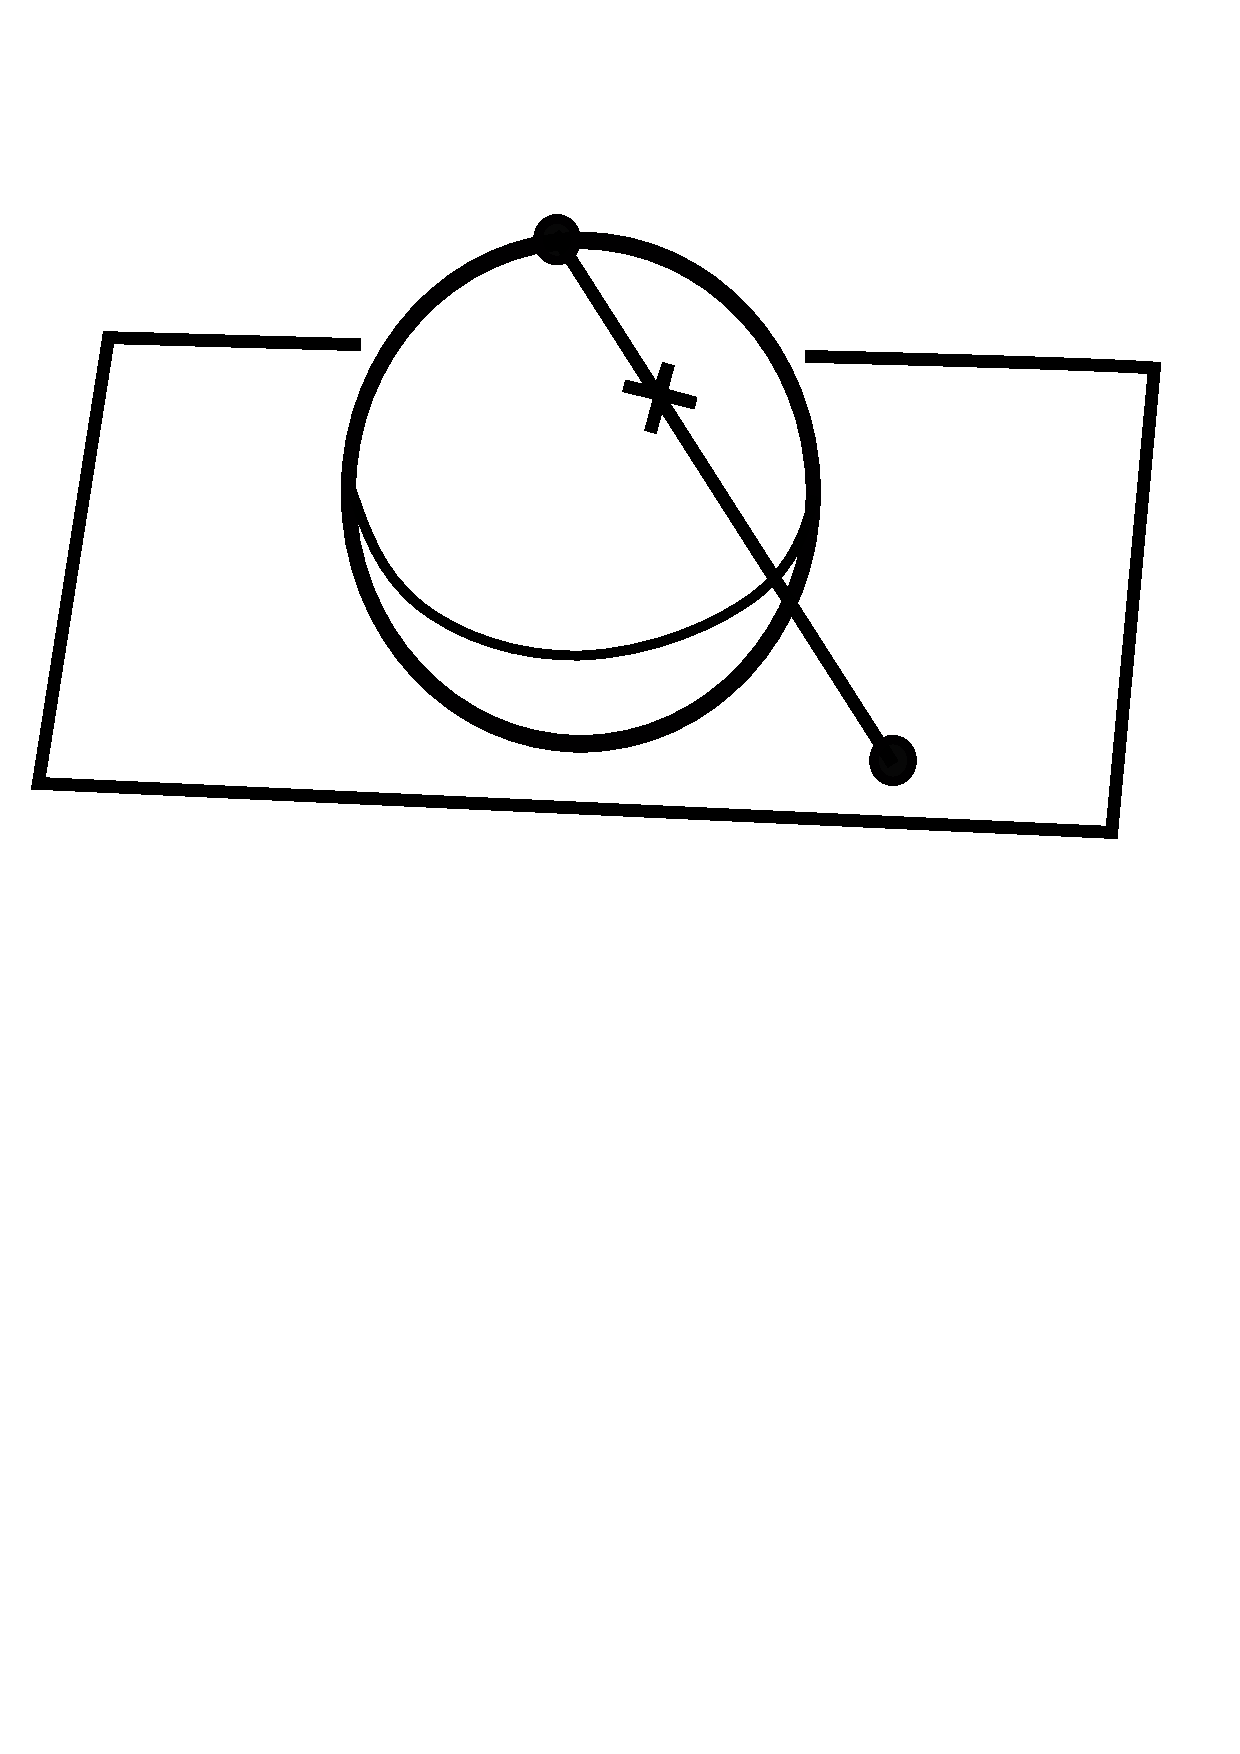
\includegraphics[width=.3\textwidth]{curvature/stereo}
	\caption{A point on the sphere is mapped to a point on the plane by stereographic projection.}
	\label{fig:stereo}
\end{figure}
	
The inverse is given by $p^{-1}:\R^2\to \R^3$

	\begin{equation}\label{eqn:stereo}
		p^{-1}(u,v)=\left(\frac{2u}{u^2+v^2+1},\frac{2v}{u^2+v^2+1},\frac{u^2+v^2-1}{u^2+v^2+1}\right).	
	\end{equation}
To compute the first fundamental form of $p^{-1}(u,v)$ we take the partial derivatives

$$p^{-1}_u=\left(\frac{2v^2-2u^2+2}{(u^2+v^2+1)^2},\frac{-4uv}{(u^2+v^2+1)^2},\frac{4v}{(u^2+v^2+1)^2}\right)$$
and 
$$p^{-1}_v=\left(\frac{-4uv}{(u^2+v^2+1)^2},\frac{2v^2-2u^2+2}{(u^2+v^2+1)^2},\frac{4v}{(u^2+v^2+1)^2}\right).$$
Then, after some algebra,
$$E=p^{-1}_u\cdot p^{-1}_u=\frac{4}{(u^2+v^2+1)^2}$$
$$F=p^{-1}_v\cdot p^{-1}_v=\frac{4}{(u^2+v^2+1)^2}$$
and
$$M=p^{-1}_u\cdot p^{-1}_v=0.$$

We can use the first fundamental form to compute
the  arc length of circles on the sphere parallel to the $xy$ plane with fixed height $z=c$ for $-1<c<1$.
This length can be computed using
the pythagorean theorem. We will see that using stereographic projection
and the first fundamental form we get the same answer.


The arc length of a parameterized curve $u=u(t), v=v(t)$ on a regular surface,
can be computed using the first fundamental form.  Let
$s$ denote the arc length, then 
$$ds=\bigg | \frac{dr}{dt}\bigg | dt = \bigg | r_u\frac{du}{dt}+r_v\frac{dv}{dt}\bigg |dt
=\sqrt{(r_u^2 du^2+2r_ur_v du dv + r_v^2dv^2)}.$$
Next, use the map $p$ to map such a circle to the plane.
Using \eqnref{stereo}, our circle on the sphere maps 
to a circle in the plane because
	$$p^{-1}(u,v)=\frac{u^2+v^2-1}{u^2+v^2+1}=c$$
and we can compute the radius in terms of $c$
\begin{equation}\label{eqn:radius}
	u^2+v^2=\frac{1+c}{1-c}=k^2.
\end{equation}
	
In the plane, $u^2+v^2=k^2$ can be parameterized
as $$\gamma(t)=(k\cos(t),k\sin(t))$$ with $0\leq t\leq 2\pi.$
So our curve becomes $p^{-1}\circ \gamma(t)$ on the sphere.
Computing the partial derivatives of $\gamma(t)$ gives
$$\gamma_u'=-k\sin(t)\hspace{1.3cm}  \gamma_v'=k\cos(t).$$
Now we use the first fundamental form

$$\int_{p^{-1}}\gamma ds=\int_{0}^{2\pi} ||(p^{-1}\circ \gamma)'(t)dt=\int_0^{2\pi}\sqrt{E(\gamma_u'(t))^2+2M\gamma_u'\gamma_v'+
F(\gamma_v'(t))^2}dt.$$
Substituting and simplifying using $E=F$ we obtain
$$\int_0^{2\pi}\frac{2k}{k^2+1}dt=\frac{4\pi k}{k^2+1}.$$
Simplifying further using \eqnref{radius}  our arc length is
$$2\pi\sqrt{1-c^2}.$$

\end{example}

\todo{Do we need this? Let $S_1$ and $S_2$ be two surfaces with $\sigma:V\subset S_1\to S_2$ a differentiable map.
At $p\in S_1$ the map $d\sigma_p:T_p(S_1)\to T_{\sigma(p)}(S_2)$ is called the
\EMPH{differential} of $\sigma$ at $p$.}


Given two curves on the sphere that intersect linearly independently at a point $p$, 
stereographic projection preserves the angle between the curves.
Maps that preserve angles in this way are called \EMPH{conformal}.

\subsubsection{Geodesics Curvature}

Shortest paths play an important role in many computational problems.
In a surface, a \EMPH{geodesic} is a curve that is a shortest path
between two points in the surface. 
For example, on $\Sp^2$ great circles are geodesic.
We would like to define the curvature of a one dimensional curve as it would
 be seen from someone living on a surface.

Let $U$ be a parameterized chart on a surface $S$ with vector $n(u,v)$ normal
to the surface
and let $\gamma(t)$ be a curve in $U$, with Frenet frame $T,N,B$.
Then $V=n(\gamma(t)\times T$ is in the tangent plane of the surface since
it is perpendicular to $n$. We now have a new orthonormal basis at a point on $\gamma$
namely, $T,V,n$. 
We would like to measure how the rate of change of the tangent vector $T$ with respect to $V$.
The \EMPH{geodesic curvature} is  
\begin{equation} \label{eqn:geodesic}
	k_g=\langle \gamma''(t),V(t)\rangle
\end{equation}
For an alternative equivalent definition see \cite{doc76}.
\todo{non great circle on sphere image}



